\documentclass[conference]{IEEEtran}
\IEEEoverridecommandlockouts
\usepackage{cite}
\usepackage{amsmath,amssymb,amsfonts}
\usepackage{graphicx}
\usepackage{booktabs}
\usepackage{xcolor}
\usepackage{url}
\usepackage[hidelinks]{hyperref}

\graphicspath{{figs/}}

\begin{document}

\title{An Intelligent Video Event Search Engine:\\
Detection--Tracking--Interval Indexing with Robust Identity Labeling}

\author{
\IEEEauthorblockN{Nikhil Singh Shekhawat \qquad Nimish Vivek Poonekar}
\IEEEauthorblockA{Khoury College of Computer Sciences, Northeastern University\\
CS~5330: Pattern Recognition and Computer Vision\\
Email: poonekar.n@northeastern.edu}
}

\maketitle

\begin{abstract}
We present an intelligent video event search engine that turns raw
footage into a searchable index of \emph{when} each object was on
screen. The system detects the 80 COCO object classes with a YOLO11
detector, assigns every object a persistent identity with ByteTrack,
and folds the per-frame boxes of each track into time intervals: one
row per appearance with a start and end timestamp. A user can then
query an object type and jump directly to the moments it appears.
Around this core we add a set of robustness and recognition passes:
adaptive low-light enhancement, per-class confidence floors,
ghost-track removal, confidence-weighted class voting, and an optional
face-recognition pass that relabels the generic ``person'' class with
an enrolled name by embedding a bounded set of face crops per track and
matching them against a gallery by cosine similarity with a margin
test. Optional passes add segmentation masks, pose-based action cues,
monocular depth, appearance re-identification, and age/gender
attributes. On a working corpus of seven videos ($\sim$21~minutes,
27{,}865 processed frames), the pipeline compresses 23{,}817 per-frame
detections into 795 interval rows---a $\sim$30$\times$ reduction---while
correctly relabeling an enrolled identity. We also describe a
quantitative evaluation harness reporting precision/recall/F1,
mAP@0.5, MOTA, IDF1, and identity accuracy.
\end{abstract}

\begin{IEEEkeywords}
object detection, multi-object tracking, video indexing, face
recognition, event search, YOLO, ByteTrack
\end{IEEEkeywords}

\section{Introduction}
Video is easy to record and hard to search. A single clip may contain
hundreds of object appearances, but a viewer usually wants a very
specific answer: \emph{when does a car appear?} or \emph{find every
moment this person is on screen}. Answering such questions by hand
means scrubbing the timeline frame by frame. The goal of this project
is to make a video searchable by \emph{content}: given any video, the
system should report, for every object it recognizes, the time
intervals during which that object was visible, and let the user query
those intervals interactively.

The task decomposes into three classical computer-vision problems and
one indexing problem. First, \textbf{detection}: identify which objects
are present in each frame and where. Second, \textbf{tracking}: link
detections of the same physical object across frames so it carries a
single persistent identifier rather than being re-counted every frame.
Third, \textbf{temporal indexing}: collapse the long, frame-indexed
stream of a track into a compact interval---a start time, an end time,
and a label---so the result is a short list of appearances rather than
a per-frame log. Finally, an interactive front end lets a user search
the index and seek to matches.

The central idea is that a \emph{persistent track identity} is the unit
that makes everything else possible. Once ``the same car'' keeps one ID
across frames, its appearance is naturally a single interval; the same
ID lets us gather a handful of crops of a person and decide their name
once; and it lets classic analytics (trajectories, occupancy, line
crossings) fall out of the box geometry for free. The remainder of this
paper describes related work (Section~\ref{sec:related}), the method in
reproducible detail (Section~\ref{sec:method}), and results on a real
corpus together with the evaluation harness
(Section~\ref{sec:experiments}).

\section{Related Work}
\label{sec:related}
Our system is an integration of several well-established lines of work;
we summarize the three most directly reused and how they relate.

\textbf{Object detection (YOLO).} Redmon \emph{et al.}~\cite{yolo}
introduced YOLO, framing detection as a single regression from image
pixels to bounding boxes and class probabilities, which made real-time,
whole-image detection practical. Our detector is a modern descendant of
this family (Ultralytics YOLO11~\cite{ultralytics}) and provides the
per-frame boxes and COCO class labels that seed every later stage. The
one-stage, real-time property is what lets us process video at
interactive rates.

\textbf{Multi-object tracking (ByteTrack).} Zhang \emph{et
al.}~\cite{bytetrack} proposed ByteTrack, which associates \emph{every}
detection box---including low-confidence ones---to existing tracks
rather than discarding weak detections before association. This
recovers objects through occlusion and motion blur and yields the
stable, long-lived track identities our interval builder depends on. We
use ByteTrack as the association layer on top of the detector. An
earlier appearance-based alternative, DeepSORT~\cite{deepsort}, augments
motion association with a learned re-identification embedding; we adopt
a similar appearance-matching idea in our optional re-ID pass.

\textbf{Face recognition (FaceNet).} Schroff \emph{et al.}~\cite{facenet}
introduced FaceNet, which learns a compact Euclidean embedding of faces
with a triplet loss so that same-identity faces are close and
different-identity faces are far apart. Our custom-identity feature
follows this embedding-and-compare recipe directly: we embed enrolled
photos and per-track face crops into a 512-d space (via an
InceptionResnetV1 backbone trained on VGGFace2~\cite{vggface2}) and
match by cosine similarity. This is what lets the generic ``person''
label be replaced by a specific enrolled name.

We additionally use monocular depth estimation for optional
distance tagging: Ranftl \emph{et al.}~\cite{midas} (MiDaS) train a
robust relative-depth network that transfers zero-shot across datasets,
which we sample sparsely to tag tracks with a coarse near/far value.
Contrast-limited adaptive histogram equalization
(CLAHE)~\cite{clahe} underlies our low-light pass.

\section{Method}
\label{sec:method}
Figure~\ref{fig:arch} shows the end-to-end pipeline. A video is read
frame by frame; each processed frame is detected and tracked; tracks
are cleaned and optionally named; and the surviving tracks are folded
into intervals that drive the search UI. All parameters below are the
defaults in our configuration and are stated so the system can be
reproduced.

\begin{figure*}[t]
\centering
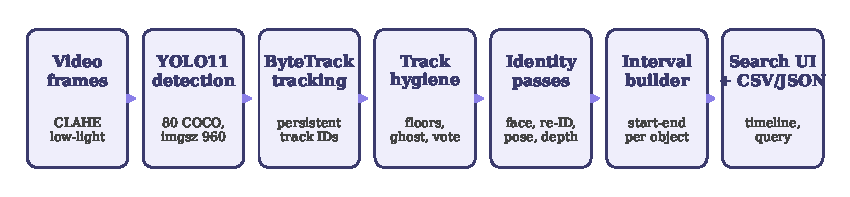
\includegraphics[width=\textwidth]{arch.pdf}
\caption{End-to-end pipeline. Each processed frame is (optionally)
contrast-enhanced, detected by YOLO11 and associated by ByteTrack into
persistent track IDs. Track-level hygiene and identity passes act once
per track, after which appearances are folded into start--end intervals
that back the search interface and the exported CSV/JSON.}
\label{fig:arch}
\end{figure*}

\subsection{Detection and preprocessing}
We use Ultralytics YOLO11-m over the 80 COCO classes at an inference
resolution of $960$~px (larger than the $640$ default to improve recall
on small and distant objects), with a tracker-facing confidence of
$0.35$ and an NMS IoU threshold of $0.5$. By default every frame is
processed (stride~$1$); a larger stride trades tracking continuity for
speed. Detection is driven through a manual capture loop (OpenCV
\texttt{VideoCapture}) so that frames can be preprocessed before
inference.

\textbf{Low-light enhancement.} A common failure mode is a back-lit or
shadowed object crushed into a silhouette, which the detector then
misclassifies. When a frame's mean luminance falls below a threshold
($90$ of $255$), we apply CLAHE~\cite{clahe} (clip limit $2.0$, $8\times8$
tiles) to the $L$ channel of the LAB representation and convert back,
restoring edges and texture. Well-lit frames (mean luma above the
threshold) are passed through untouched, so the cost is paid only where
it helps.

\subsection{Tracking and track-level hygiene}
Detections are associated across frames by ByteTrack~\cite{bytetrack}
(Ultralytics \texttt{bytetrack.yaml}) with \texttt{persist=True} so
tracker state carries across our manual per-frame calls. Each surviving
box thus receives a persistent \texttt{track\_id}. Three passes then
clean the tracks:
\begin{itemize}
  \item \textbf{Per-class confidence floors.} A detection is kept only
  if its confidence clears a floor for its class ($0.40$ by default,
  $0.50$ for \texttt{person}, which is the class most often hallucinated
  from silhouettes and animals). This filtering happens after tracking
  so ByteTrack still sees weak boxes for association.
  \item \textbf{Ghost-track removal.} A track seen in fewer than $3$
  kept frames is discarded, eliminating momentary false detections that
  never recur.
  \item \textbf{Confidence-weighted class voting.} Every track is
  relabeled to the class it was assigned most often, weighted by
  confidence, so a single-frame flicker to the wrong class is corrected
  across the whole appearance.
\end{itemize}

\subsection{Identity labeling by face recognition}
When at least one person has been enrolled, the ``person'' class can be
replaced by a specific name. Enrollment stores one $512$-d, $L_2$-normalized
face embedding per uploaded photo, computed with an MTCNN face detector
and an InceptionResnetV1/VGGFace2 backbone (facenet-pytorch), following
the FaceNet embedding recipe~\cite{facenet,vggface2}.

Enrolled embeddings persist on disk (one \texttt{.npy} matrix and a
thumbnail per person) and are loaded once into a single cached gallery
matrix; a match is a matrix product of the $L_2$-normalized gallery with
a query embedding, reduced to the best cosine score per enrolled name.

During analysis we do \emph{not} run face inference every frame. Instead,
for each person track we keep at most $8$ crops chosen by
$\text{area}\times\text{confidence}$ (rejecting crops smaller than
$40\times60$~px). After the main loop, each kept crop is embedded and
matched against the gallery: a crop counts for a name only if its cosine
similarity is at least $0.55$ \emph{and} exceeds the best competing
enrolled name by a margin of $0.05$ (an ambiguous match is left as
``person''), and only faces with MTCNN probability $\ge 0.92$ are
embedded at all. The per-crop votes are tallied and the track is renamed
only if the winning name receives at least $2$ votes. Because this runs a
handful of times per track rather than per frame, its cost is bounded and
the whole appearance gets a single, stable name.

\subsection{Optional perception passes}
The same per-track crop store and tracking scaffold support several
optional passes, each disabled by default:
\emph{segmentation} swaps in the YOLO11-seg variant so each detection
also carries a simplified polygon mask;
\emph{pose} runs a YOLO11-pose model, associates its 17 keypoints to
person boxes by IoU ($>0.3$), and reduces them to a coarse action
(standing/sitting/fallen/raising-hand);
\emph{monocular depth} runs MiDaS-small~\cite{midas} (loaded via
\texttt{torch.hub}) on $8$ frames sampled across the video and tags each
track with the median relative depth ($0=$far, $1=$near) inside its box;
\emph{appearance re-ID} embeds each person track's crops with an ImageNet
ResNet-50 encoder (a $2048$-d $L_2$-normalized global-average-pooled
feature from a $128\times256$ crop) and propagates a face-derived name to
an unnamed person track whose mean-appearance cosine similarity exceeds
$0.82$, carrying an identity across a broken track or a turned-away
stretch; and \emph{attributes} estimates age and gender per person track
with InsightFace (buffalo\_l) on CPU via ONNX Runtime.

\subsection{Interval construction}
The core index is built by a single ordered scan over the cleaned
frames. For each track we maintain a running end time that is pushed
forward while the track remains visible. When a track has been absent
for longer than a gap tolerance of $0.6$~s---which absorbs brief
occlusions and missed detections so one car behind a pole is not split
into many rows---its interval is finalized. Appearances shorter than
$0.3$~s are dropped as noise. Each finalized interval records the track
ID, voted class (or name), start/end in both seconds and
\texttt{HH:MM:SS.mmm}, duration, and peak confidence. Intervals are
written to CSV and JSON; a per-class rollup counts distinct objects and
total appearances.

\subsection{Analytics and system}
Because every object has a track, classic analytics are computed from
box geometry alone: per-track trajectories, distance/speed/heading,
an occupancy heatmap of foot points (Gaussian-blurred, JET-colormapped),
and directional line crossings at mid-frame (people/traffic counting).
The system is served by a FastAPI backend that accepts an upload, runs
processing in a background job with progress reporting, and exposes
per-class summary, interval search, per-frame detections, and byte-range
video streaming to a browser front end that draws live tracking overlays
and a searchable object timeline. A headless CLI
(\texttt{process\_video.py}) runs the identical pipeline without the UI,
writing \texttt{detections.json}, \texttt{intervals.csv}, and
\texttt{summary.json} for testing and batch use.

\subsection{Evaluation harness}
For quantitative measurement, an evaluation module scores the stored
predictions against a hand-labeled ground-truth (GT) JSON aligned by
nearest timestamp. \textbf{Detection} uses greedy, per-class, IoU-$\ge0.5$
matching in descending confidence to compute precision, recall, F1, and
average precision (AP@0.5, averaged over classes to give mAP@0.5).
\textbf{Tracking} reports MOTA and IDF1 via \texttt{motmetrics} when the
GT carries per-object IDs. \textbf{Identity} reports the fraction of
named GT person boxes whose matched prediction carries the correct
enrolled name. These metrics let detection, tracking, and recognition
quality be reported separately.

\section{Experiments and Results}
\label{sec:experiments}
\subsection{Corpus and protocol}
We evaluated the system on a working corpus of seven processing runs
spanning roughly $21$~minutes of footage at resolutions up to
$1920\times1080$ and $25$--$30$~fps (Table~\ref{tab:corpus}); two runs
are re-processings of the same maritime source and are therefore
identical. In total $27{,}865$ frames were processed. All runs used the
default configuration of Section~\ref{sec:method} on an NVIDIA RTX~5060
GPU. Reported quantities are read directly from the artifacts the
pipeline writes (\texttt{summary.json}, \texttt{detections.json}).

\begin{table}[t]
\caption{Per-run corpus statistics (as processed).}
\label{tab:corpus}
\centering
\footnotesize
\setlength{\tabcolsep}{3.2pt}
\begin{tabular}{lrrrrr}
\toprule
run & dur~(s) & resolution & frames & det.\ inst. & intervals \\
\midrule
0840fd & 289.9 & 1920$\times$1080 & 7248 & 4362 & 153 \\
0a1cdc & 57.0  & 1920$\times$1080 & 1709 & 6198 & 174 \\
1c3ecb & 289.9 & 1920$\times$1080 & 7248 & 4362 & 153 \\
398493 & 289.9 & 1920$\times$1080 & 7248 & 5178 & 159 \\
54451f & 11.9  & 1024$\times$576  & 359  & 1758 & 55  \\
62bb27 & 289.8 & 1920$\times$1080 & 3624 & 1712 & 91  \\
7067be & 29.0  & 940$\times$560   & 429  & 247  & 10  \\
\midrule
total & 1257.4 & --- & 27865 & 23817 & 795 \\
\bottomrule
\end{tabular}
\end{table}

\subsection{Result 1: interval compression}
The system's core claim is that a per-frame detection stream can be
reduced to a compact, searchable set of appearances. Across the corpus,
$23{,}817$ per-frame detection instances were folded into $795$ interval
rows---a $\mathbf{30\times}$ reduction in the number of records a user
must reason about, with no loss of the ``when did it appear'' answer.
Figure~\ref{fig:compress} shows the reduction is consistent across runs
of very different length and density. This is the quantitative
expression of the design goal: search over appearances, not frames.

\begin{figure}[t]
\centering
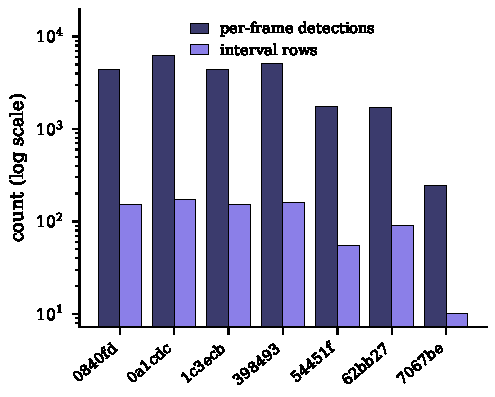
\includegraphics[width=\columnwidth]{compress.pdf}
\caption{Per-frame detections vs.\ interval rows for each run (log
scale). Every run is compressed by roughly an order of magnitude or
more; the aggregate reduction is $30\times$.}
\label{fig:compress}
\end{figure}

\subsection{Result 2: class coverage}
Across the corpus the pipeline produced tracked objects in $37$ distinct
COCO classes. Figure~\ref{fig:classes} shows the distribution is
dominated by \texttt{person}, \texttt{boat}, and \texttt{bird},
consistent with the maritime and street scenes in the footage, with a
long tail of vehicles, animals, and everyday objects
(\texttt{car}, \texttt{dog}, \texttt{backpack}, \texttt{traffic light},
\ldots). The breadth confirms the index is populated from the full COCO
label set rather than a handful of easy categories.

\begin{figure}[t]
\centering
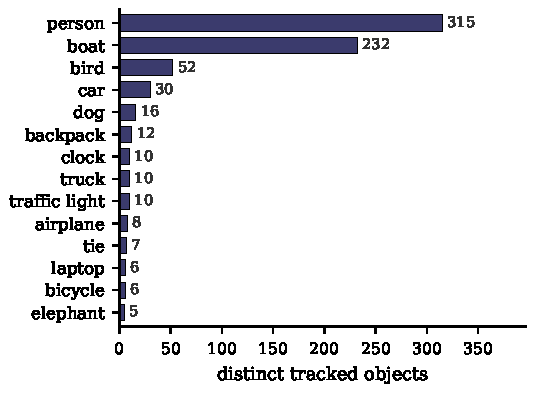
\includegraphics[width=\columnwidth]{classes.pdf}
\caption{Distinct tracked objects per class (top~14 of 37 classes
observed across the corpus).}
\label{fig:classes}
\end{figure}

\subsection{Result 3: identity relabeling}
With a single enrolled person in the gallery, the face-recognition pass
correctly replaced the generic label on the matching person track in
run \texttt{54451f}: that run's rollup contains $45$ \texttt{person}
appearances plus one appearance labeled with the enrolled name, rather
than $46$ anonymous people. This demonstrates the embedding-match-vote
path end to end---enrollment, bounded per-track crop sampling, cosine
matching with a margin test, and majority voting---renaming a whole
appearance from a handful of crops.

\subsection{Robustness behavior}
The track-hygiene passes act directly on the statistics above. The
person-class confidence floor ($0.50$ vs.\ the $0.40$ default) suppresses
the silhouette-to-person errors that are common in the back-lit maritime
footage; ghost-track removal ($\ge3$ detections) prevents momentary
false positives from ever becoming intervals; and confidence-weighted
voting guarantees each interval carries one stable class even when a
track briefly flickers between labels. Together these convert noisy
per-frame detections into clean, trustworthy appearances---the
difference between a raw detector log and a searchable index.

\subsection{Discussion and limitations}
Our results are system- and corpus-level: they demonstrate that the
pipeline runs end to end at interactive rates, compresses detections
into a faithful interval index, spans the full label set, and performs
identity relabeling. We do \emph{not} yet report detection/tracking
accuracy against a large labeled benchmark; the evaluation harness of
Section~\ref{sec:method} provides precision/recall/F1, mAP@0.5, MOTA,
IDF1, and identity accuracy, but a bundled ground-truth set is future
work (a labeled subset of ActivityNet or Kinetics is the intended
target). The interval builder also inherits the detector's and tracker's
errors: a persistent ID switch would split one appearance into two
intervals, and a systematically missed class would simply be absent from
the index.

\section{Conclusion}
We built an intelligent video event search engine that indexes footage
by \emph{when} each object appears. Detection (YOLO11) and tracking
(ByteTrack) produce persistent object identities, which are cleaned by
confidence floors, ghost removal, and class voting, optionally named by
a bounded face-recognition pass, and folded into compact time intervals
that a user can search interactively. On a real corpus the pipeline
achieved a $30\times$ reduction from detections to searchable
appearances across $37$ classes while correctly relabeling an enrolled
identity, and it ships with an evaluation harness for detection,
tracking, and identity metrics. Future work is a large-scale labeled
evaluation, export of matched clips, and open-vocabulary queries for
objects outside the COCO label set.

\begin{thebibliography}{1}
\bibitem{yolo}
J.~Redmon, S.~Divvala, R.~Girshick, and A.~Farhadi, ``You Only Look
Once: Unified, Real-Time Object Detection,'' in \emph{Proc.\ IEEE Conf.\
Computer Vision and Pattern Recognition (CVPR)}, 2016, pp.~779--788.

\bibitem{bytetrack}
Y.~Zhang, P.~Sun, Y.~Jiang, D.~Yu, F.~Weng, Z.~Yuan, P.~Luo, W.~Liu, and
X.~Wang, ``ByteTrack: Multi-Object Tracking by Associating Every
Detection Box,'' in \emph{Proc.\ European Conf.\ Computer Vision
(ECCV)}, 2022, pp.~1--21.

\bibitem{deepsort}
N.~Wojke, A.~Bewley, and D.~Paulus, ``Simple Online and Realtime
Tracking with a Deep Association Metric,'' in \emph{Proc.\ IEEE Int.\
Conf.\ Image Processing (ICIP)}, 2017, pp.~3645--3649.

\bibitem{facenet}
F.~Schroff, D.~Kalenichenko, and J.~Philbin, ``FaceNet: A Unified
Embedding for Face Recognition and Clustering,'' in \emph{Proc.\ IEEE
Conf.\ Computer Vision and Pattern Recognition (CVPR)}, 2015,
pp.~815--823.

\bibitem{vggface2}
Q.~Cao, L.~Shen, W.~Xie, O.~M. Parkhi, and A.~Zisserman, ``VGGFace2: A
Dataset for Recognising Faces across Pose and Age,'' in \emph{Proc.\
IEEE Int.\ Conf.\ Automatic Face and Gesture Recognition (FG)}, 2018,
pp.~67--74.

\bibitem{midas}
R.~Ranftl, K.~Lasinger, D.~Hafner, K.~Schindler, and V.~Koltun,
``Towards Robust Monocular Depth Estimation: Mixing Datasets for
Zero-Shot Cross-Dataset Transfer,'' \emph{IEEE Trans.\ Pattern Anal.\
Mach.\ Intell.}, vol.~44, no.~3, pp.~1623--1637, 2022.

\bibitem{clahe}
K.~Zuiderveld, ``Contrast Limited Adaptive Histogram Equalization,'' in
\emph{Graphics Gems IV}. San Diego, CA, USA: Academic Press, 1994,
pp.~474--485.

\bibitem{ultralytics}
G.~Jocher and J.~Qiu, ``Ultralytics YOLO11,'' 2024. [Software].
Available: \url{https://github.com/ultralytics/ultralytics}

\end{thebibliography}

\end{document}
